\input preamble_DPO_xe.tex

\date{27 января 2021}		% Дата семинара
\setcounter{s}{3}			% Номер семинара

\begin{document}


\title{Дискретная математика:\\
неориентированные графы}

\institute{Факультет компьютерных наук, НИУ ВШЭ}

\begin{frame}
  \titlepage
\end{frame}


\begin{frame}{Графы -- мотивировка}

\exmpl Между девятью планетами Солнечной системы введено космическое сообщение. Ракеты летают по следующим маршрутам: Земля --- Меркурий, Плутон --- Венера, Земля --- Плутон, Плутон --- Меркурий, Меркурий --- Венера, Уран --- Нептун, Нептун --- Сатурн, Сатурн --- Юпитер, Юпитер --- Марс и Марс --- Уран.

Можно ли добраться с Земли до Марса?

\end{frame}


\begin{frame}{Определение неориентированного графа}

Неформально, \acc{граф} --- это пара множества \acc{вершин} и множества \acc{ребер}.

Рассмотрим произвольное множество вершин $V$.

Ребра удобно рассматривать как множество пар вершин $$E\subseteq \{\ \{v,u\}\ |\ u,v \in V\}.$$
\defn \acc{Графом} называется пара $G=(V,E)$.



\end{frame}


\begin{frame}{Базовые определения теории графов}

\defn Вершина и ребро \acc{инцидентны}, если вершина является концом этого ребра.

\defn \acc{Петля} в графе --- ребро, инцидентное одной и той же вершине. 

\defn Два ребра, имеющие общую концевую вершину, называются \acc{смежными}.

\defn \acc{Изолированной вершиной} --- вершину, не инцидентная ни одному ребру.

\defn \acc{Степенью} вершины $v$ называется количество инцидентных ей ребер. Обозначение: $\deg v.$

\end{frame}


\begin{frame}{Полный граф}

\centerline{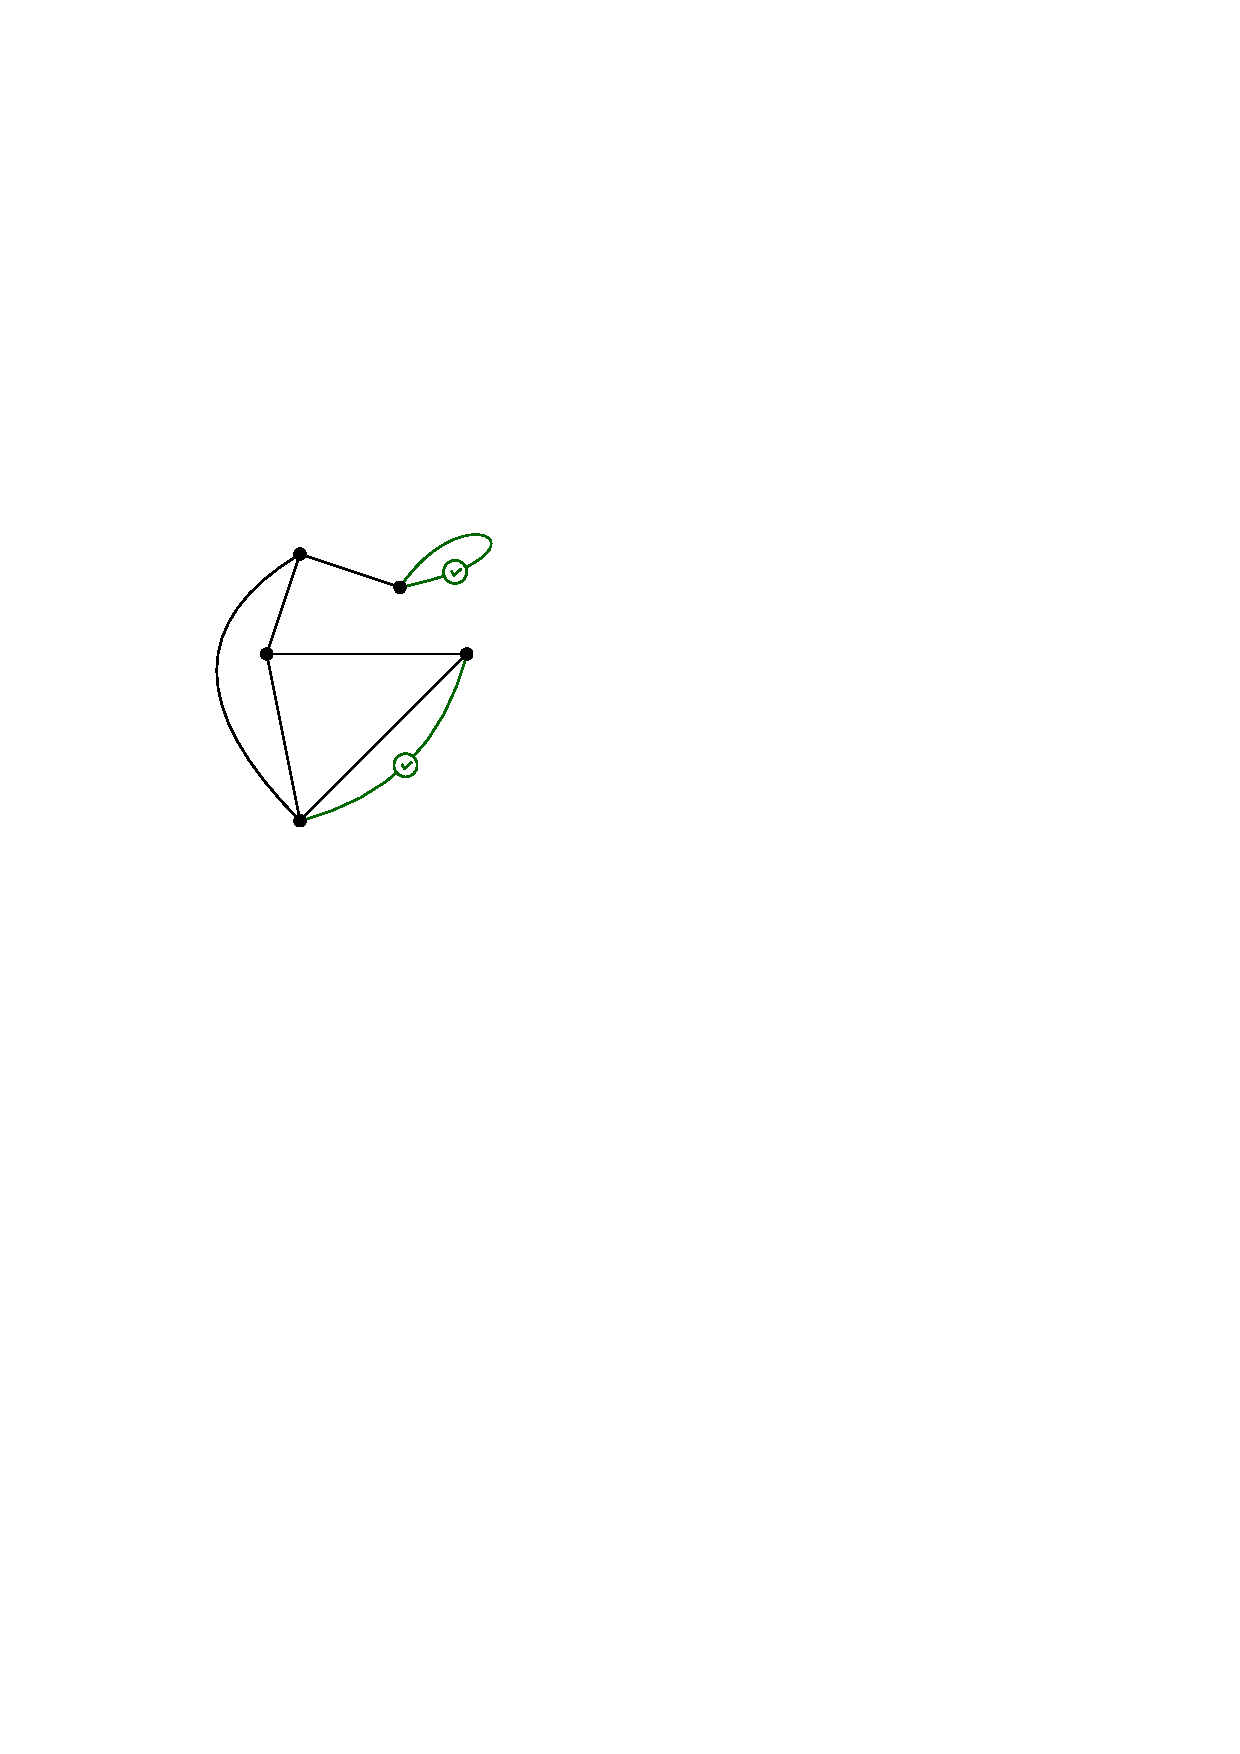
\includegraphics[scale=0.7]{img/graph02.pdf} \qquad 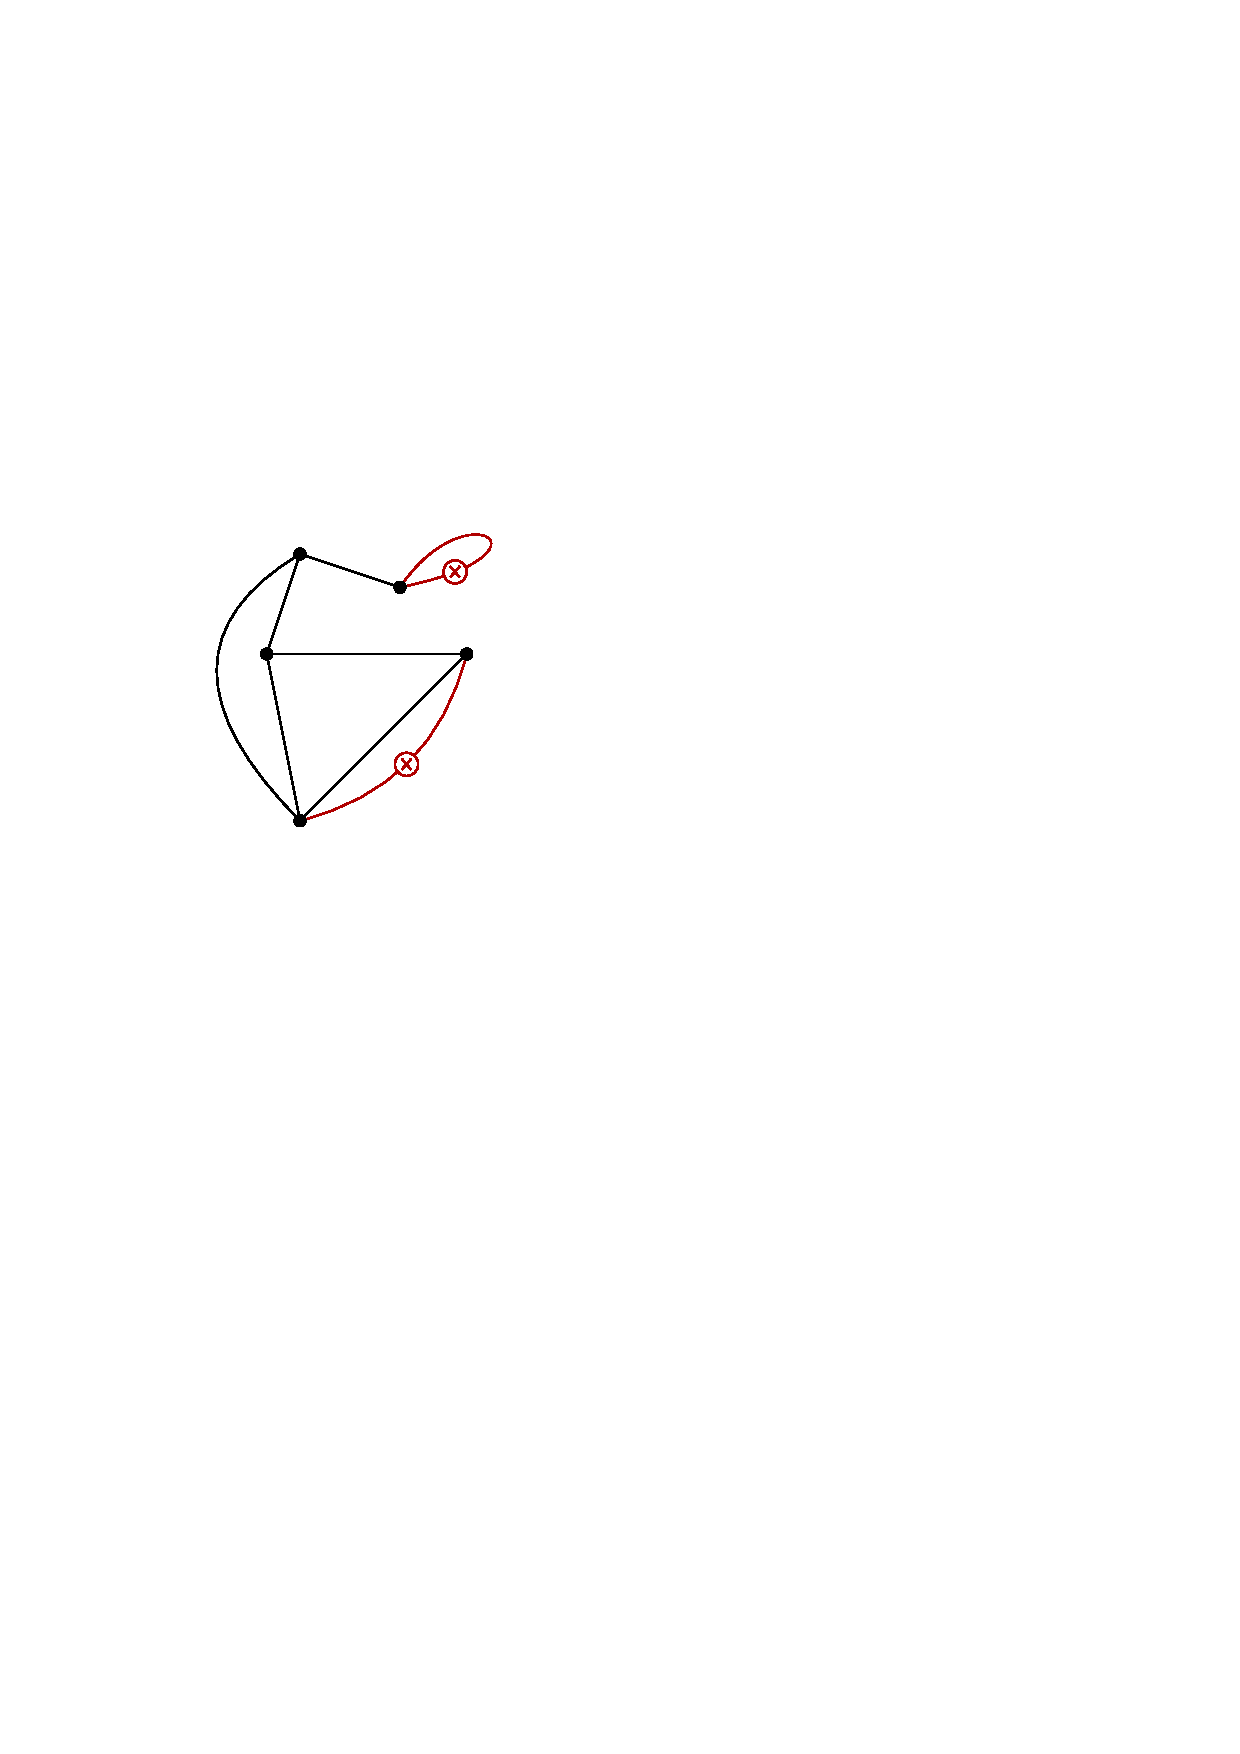
\includegraphics[scale=0.7]{img/graph01.pdf}}

Далее на этой лекции мы будем рассматривать графы \acc{без петель} и \acc{кратных ребер}.

\defn Граф на $n$ вершинах называется \acc{полным}, если в нём каждая вершина
соединена с каждой. Обозначение $K_n$.
\spc

{\bf Утверждение.} В полном графе $K_n$ ровно $\frac{n(n-1)}{2}$ ребер.

\end{frame}

\begin{frame}{Лемма о рукопожатиях}

{\bf Лемма (О рукопожатиях).} Сумма степеней всех вершин графа равна удвоенному числу ребер:
$$\sum_{v_i\in V}\deg v_i=2|E|.$$

\exmpl У кого в среднем больше партнеров противоположного пола? У мужчин или у женщин?
\spc

The Social Organization of Sexuality
\spc

https://press.uchicago.edu/ucp/books/book/chicago/S/bo3626005.html

\end{frame}

\begin{frame}{Пути и циклы}

\defn \acc{Путём} в графе называют последовательность вершин $u_1 ,u_2 ,\ldots,u_n$, в которой каждые две соседние вершины соединены ребром.

\defn \acc{Длиной пути} называют количество рёбер пути (если в пути $n$ вершин, то его длина $n-1$).

\defn \acc{Циклом} в неориентированном графе называют путь длины не меньше трёх, начальная и конечная вершина которого совпадают.

\defn Путь называют \acc{простым}, если все его вершины различны.

\defn Цикл называют \acc{простым}, если все вершины цикла кроме $u_1$ и $u_n$ различны.

\end{frame}

\begin{frame}{Эйлеровы пути и циклы}

\acc{Эйлеров путь} в графе --- это путь, проходящий по всем рёбрам графа ровно по одному разу.
\spc

\acc{Эйлеров цикл} --- эйлеров путь, являющийся циклом.

\end{frame}

\begin{frame}{Эйлеровы пути и циклы}

\exmpl (Задача Эйлера о кёнигсбергских мостах.) Город Кёнигсберг (ныне Калининград) был расположен на берегах реки Прегель и двух островах, которые соединены семью мостами. Можно ли было прогуляться по городу, пройдя по каждому мосту ровно один раз, так, чтобы маршрут начался и закончился на берегу?

\centerline{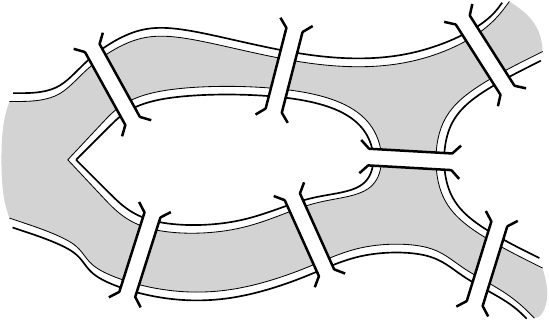
\includegraphics[scale=0.4]{img/euler2.png}}

\end{frame}

\begin{frame}{Эйлеровы пути и циклы}

{\bf Теорема 1 (Критерий существования эйлерова цикла).} В графе $G=(V,E)$ существует эйлеров цикл тогда и только тогда, когда все вершины имеют четную степень.

\spc
{\bf Теорема 2 (Критерий существования эйлерова пути).} В графе $G=(V,E)$ существует эйлеров путь тогда и только тогда, когда количество вершин с нечетной степенью меньше или равно двум.

\end{frame}

\begin{frame}{Связность}

\defn Говорят, что вершина $v$ \acc{достижима} из вершины $u$, если в графе есть
путь из $u$ в $v$. 

\defn Множество состоящее из попарно достижимых вершин называют \acc{компонентой связности}.

\defn Граф называется \acc{связным}, если он содержит ровно одну компоненту связности.

\exmpl Пусть $G$ --- граф на $15$ вершинах, причем каждая имеет степень не меньше $7$. Докажите, что $G$ связен.

\exmpl Найдите наибольшее возможное число ребер в несвязном графе на $n$ вершинах.

\end{frame}

\begin{frame}{Деревья}

\defn Связный граф без простых циклов называется \acc{деревом}.

\spc
{\bf Утверждение.} В любом дереве есть вершина степени $1$ ("висячая вершина" или "лист").

\spc
{\bf Утверждение.} У  любого дерева ровно $|V|-1$ ребро.

\vspace{5 pt}
\exmpl Существует ли дерево на $9$ вершинах, из которых хотя бы $2$ имеют степень $5$?

\end{frame}

\begin{frame}{Остовное дерево}

\defn Пусть $G$ некоторый связный граф. Подграф, являющийся деревом и содержащий все вершины называется \acc{остовным деревом} графа $G$.

\spc
{\bf Утверждение.} У  любого связного графа есть остовное дерево.

\exmpl В каждом связном графе есть такая вершина, что если ее удалить (вместе со
всеми исходящими из нее ребрами), то граф останется связным.


\end{frame}

\begin{frame}{Дополнение графа}{Дополнительный материал}

\defn \acc{Дополнением} $\bar{G}$ графа $G$ называется граф на том же множестве вершин, в котором пара вершин связана ребром тогда и только тогда, когда в $G$ эта пара вершин ребром не связана.


\exmpl Докажите, что граф или его дополнение связны (возможно оба связны).


\end{frame}



\begin{frame}{Разрезы}{Дополнительный материал}

\defn \acc{Разрезом} в графе называют разбиение множества вершин графа $V$
на множества $S$ и $T$ (которые не пересекаются). То есть $V = S \cap T$,
$S \cap T = \varnothing$.

\defn \acc{Величиной (или размером) разреза} называют суммарное
количество рёбер, которые ведут из вершин множества $S$ в вершины
множества $T$.

\end{frame}

\begin{frame}{Разрезы}{Дополнительный материал}

\centerline{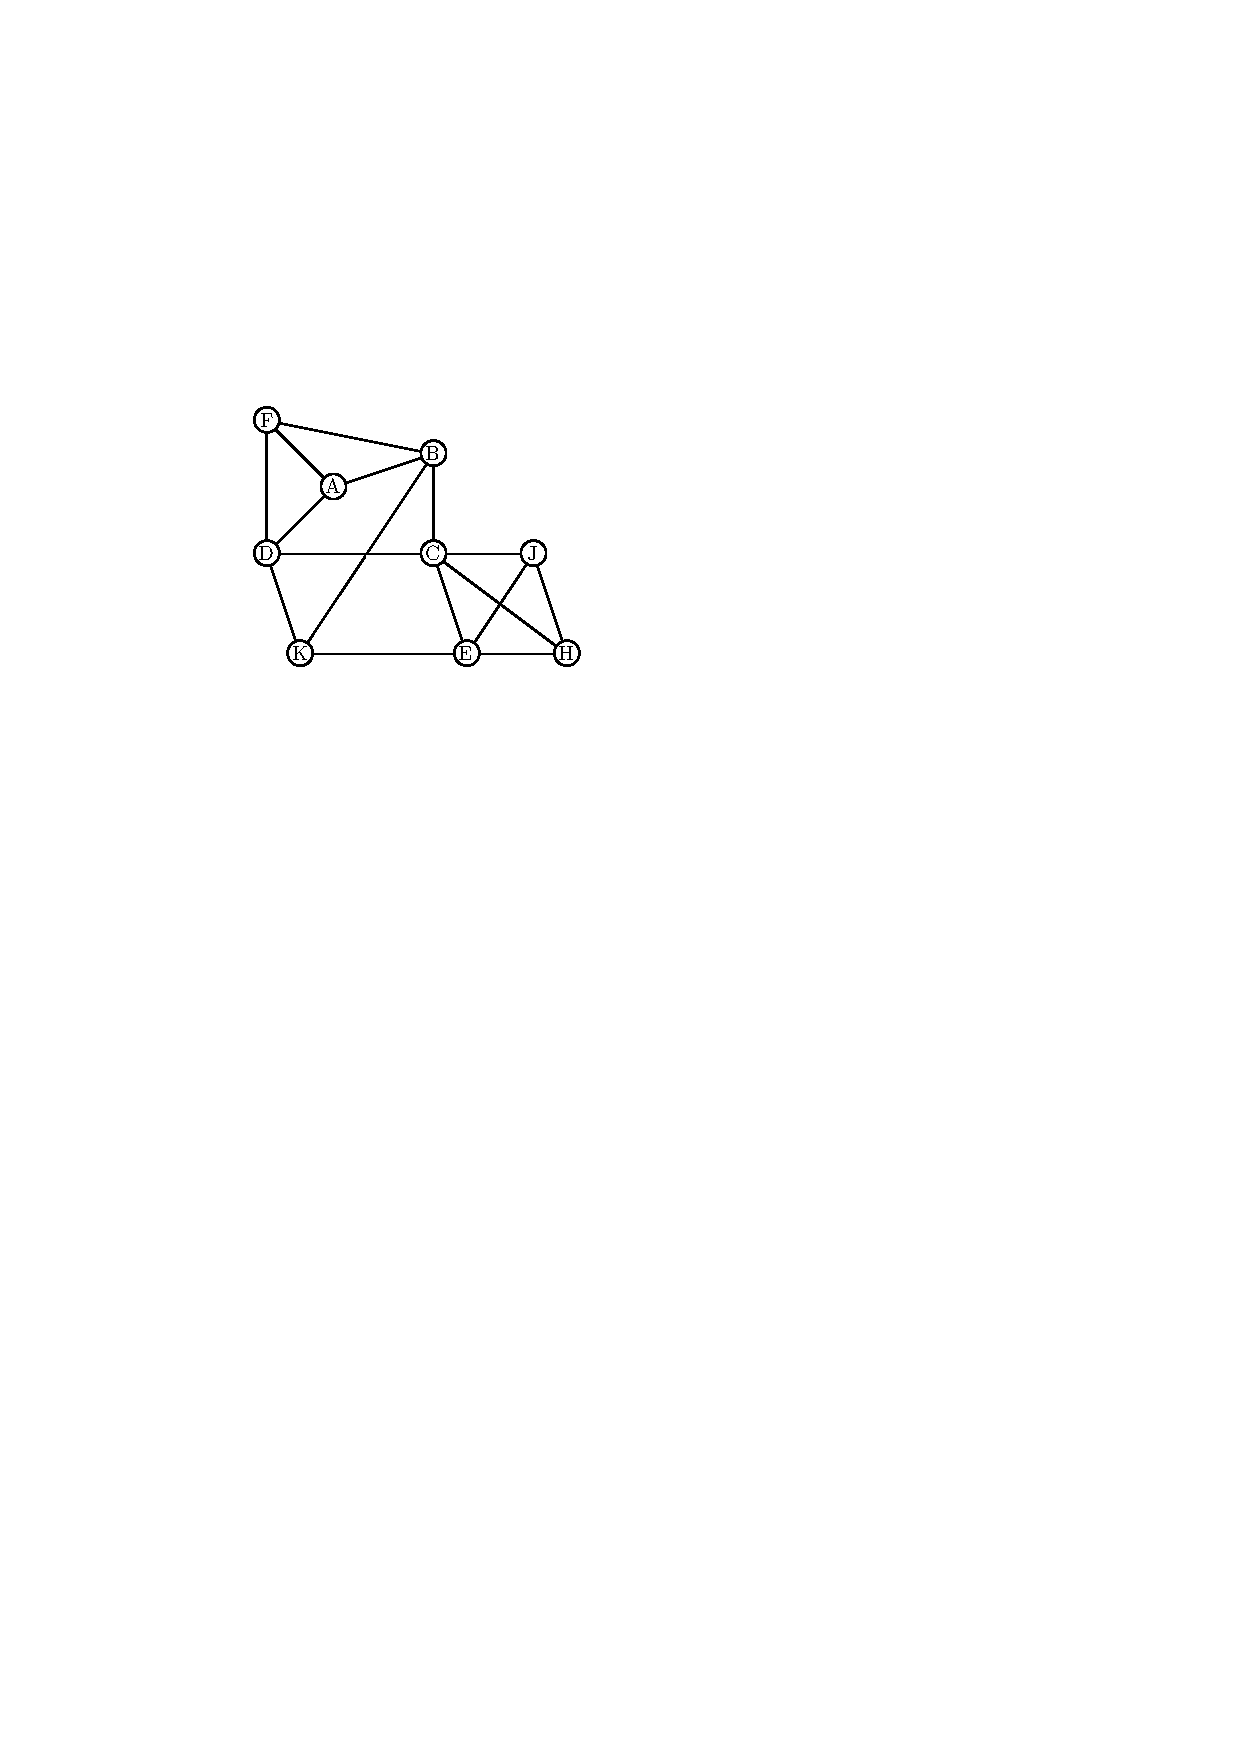
\includegraphics[scale=0.6]{img/graph1.pdf}}

\exmpl Найдите в графе $G$ разрез размера $6$. Есть ли в графе
$G$ разрез большего размера?
\spc

Из определения следует, что количество рёбер в минимальном разрезе
неориентированного графа --- это количество рёбер, которое необходимо
удалить, чтобы граф стал несвязным.

\exmpl Найдите минимальный разрез графа $G$. Докажите,
что найденный разрез действительно минимальный.

\end{frame}

\begin{frame}{Семинарская часть}

\z Найдите число рёбер в графе $K_5$.

\z Найдите число путей и простых путей длины $4$ в графе~$K_5.$ Тот же вопрос для путей длины $5$.

\z Докажите, что не существует графа с пятью вершинами, степени которых равны $4, 4, 4, 4, 2.$

\z В графе $100$ вершин и $800$ рёбер. Докажите, что в этом графе есть
хотя бы одна вершина степени не меньше $16.$

\end{frame}

\begin{frame}{Семинарская часть}

\z Дерево имеет $2020$ вершин. Верно ли, что в нём найдется простой путь
длины $3$?

\z В дереве нет вершин степени $2$. Докажите, что количество висячих
вершин (т.е. вершин степени $1$) больше половины общего количества вершин.

\z У связного графа на $10$ вершинах $15$ ребер. Какое максимальное число ребер можно удалить из него так, чтобы он остался связным?

\end{frame}



\end{document}


